% sage_latex_guidelines.tex V1.01, 11 June 2015

\documentclass[Afour,sageh,times]{sagej}


\usepackage{moreverb,url}

\usepackage[colorlinks,bookmarksopen,bookmarksnumbered,citecolor=red,urlcolor=red]{hyperref}

\newcommand\BibTeX{{\rmfamily B\kern-.05em \textsc{i\kern-.025em b}\kern-.08em
T\kern-.1667em\lower.7ex\hbox{E}\kern-.125emX}}

\def\volumeyear{2015}

\begin{document}

\runninghead{Garc\'ia-S\'anchez et al.}

\title{Parallel Multi-objective optimization using co-evolutionary islands and search space overlapping}

\author{Pablo Garc\'ia-S\'anchez, Julio Ortega, Jes\'us Gonz\'alez, Pedro Angel Castill and Juan Juli\'an Merelo\affilnum{1}}

\affiliation{\affilnum{1}Dept. of Computer Architecture and Computer Technology, University of Granada, Spain}

\corrauth{Pablo Garc\'ia-S\'anchez,
ETS. Ingenierías en Inform\'atica y Telecomunicaci\'on and CITIC-UGR,
C/Periodista Daniel Saucedo s/n,
Universidad de Granada,
18071, Granada, Spain.}

\email{pablogarcia@ugr.es}

\begin{abstract}
This paper...
\end{abstract}

\keywords{Multi-objective algorithms, NSGA-II, Island model, distributed evolutionary algorithms}

\maketitle

\section{Introduction}


%Evolutionary Algorithms (EAs) are inherently parallelizable, as each
%individual can be considered as an independent unit
%\cite{Alba13parallel}, and therefore, the
%computational performance can be improved over their non-parallel
%versions. This can also be applied to Multi-Objective Evolutionary 
%Algorithms (MOEAs). Besides, as this kind of algorithms may be computationally
%expensive, several parallelization methods have been proposed
%\cite{Luna15Survey}. However, as MOEAs deal with whole solution sets
%called Pareto Fronts (PFs), different distribution and sharing
%mechanisms need to be addressed, as there exist a tension between 
%the speedup achievable from parallelization and the need to globally 
%recombine results to accurately identify the PF \cite{Branke04Parallelizingcone}.
%
%
%Classic approaches, such as the
%global parallel EAs (Master-Slave), or the spatially structured
%algorithms (Island model or Cellular EAs) have been applied successfully in the past \cite{Folino03cellular,Alba02Parallelism}.  
%
%MOEAs have gained attention in the last years, mostly because their application in real-world problems \cite{Luna15Survey,Mukhopadhyay14Survey}. Usually these problems require a higher number of decision variables, and these larger individuals require a significant extra time for crossover, mutation and transmission. Therefore, dividing the decision space (that is, the chromosome) may improve high performance and solution quality. In this aspect, the co-%evolution model is a dimension-distributed model where a
%high-dimensional problem is divided into lower dimensional problems
%\cite{Gong15models}, and evolved separately. Also, applying parallelism techniques in EAs not only implies a reduction in the execution time, 
%but developing new and more efficient search models \cite{Luna15Survey}.  The idea of dividing the decision space has been
%studied in \cite{Kimovski15Parallel}. In that work, different workers
%evolve sub-populations created and recombined by a master process,
%which performs different recombination alternatives from the parts returned by
%worker processes. A high dimensional problem was used to compare these
%alternatives. In \cite{Dorronsoro13superlinear}, a distributed coevolutionary island model was used.  In both previous works
%significant speedups were attained, although only a low number of nodes were used (8). However, when increasing the number of islands, the division of %each section of the chromosome becomes smaller, and the scalability may be affected by obtaining lower quality solutions in the same amount of time.
%
%
%The hypothesis of this paper is that using overlapped sections of the chromosome in a coevolutionary multi-objective island-based algorithm can improve %the quality of the
%solutions in the same computing time when the number of islands increases. To demonstrate this, a new overlapping islands scheme will be compared with a baseline version of a distributed NSGA-II \cite{Deb00NSGAII} and with a coevolutionary disjoint section approach, in different benchmarks problems and %with different large number of islands. Results show that this new technique can improve different quality indicators in
%the same amount of time. 
%
%The rest of the paper is structured as follows: after a background in parallelization in MOEAs, 
 %the compared algorithms and the used methodology (Section \ref{sec:met}) are presented. 
%Then, the results of the experiments are shown (Section \ref{sec:res}), followed by conclusions and suggestions for future work lines.


%%%%%%%%%%%%%%%%%%%%%%%%%%%%%%  STATE OF THE ART  %%%%%%%%%%%%%%%%%%%%%%%%%%%%%
%
\section{State of the Art}
\label{sec:soa}


%Distributed and parallel Evolutionary Algorithms have been used since
%the early 2000s \cite{Talbi08Parallel} to leverage the capabilities of new common parallel computer architectures, such as
%clusters or grids. However, distributing MOEAs is not as easy as it is
%in single-objective EAs, as they have to deal with a whole set of dependent solutions, the Pareto Front, that should be managed in several steps of the %algorithm. %unfinished Pablo: Done
%Some authors have focused on Master-Slave approaches to parallelize this kind of EAs. For example, Durillo et
%al. \cite{Durillo08masterslave} compared different master-slave
%approaches to save time when running the EA. The method proposed by
%Hiroyasu \cite{Hiroyasu07discussion} generates offspring depending on
%the computation power.  
%
%
%
%First approaches for distributed MOEAs (dMOEAs) were studied in
%\cite{Deb03distributed}. In that work, the dominance of solutions is
%divided in the islands using a transformation of coordinates. Authors
%concluded that dividing the search space is a good idea, but achieve
%this is not trivial. Other ideas for dividing the search space include
%objective separation in different processors \cite{Xiao03specialized},
%or divide in two populations: one for elite and other search
%\cite{Wang09parallel}. Martens, in \cite{Martens13asynchronous} generated a
%Barabasi-Albert network as the island topology, and selection based on migrating
%individuals from a not-crowded area and acceptance based on
%diversity. 
%
%More similar approaches to the one presented here were studied in the
 %next two works, also using cooperative coevolution for high-dimensional problems. Dorronsoro et al. in
%\cite{Dorronsoro13superlinear} obtained super-linear performance
%in several instances using cooperative coevolution, focusing each island on a portion of the chromosome. However, in some instances the parallel version %not always 
%improved the sequential version.  Kimovski et al. \cite{Kimovski15Parallel} proposed a
%master-slave method that splits the population into several processors,
%each one running in parallel a MOEA that only affects some portion of
%the individuals. After a certain number of generations, the master
%process receives all the sub-populations to be combined. Different
%combination alternatives in this step are compared. Up to 8 processors
%were used in the experimental setup. Our approach in this paper does not
%broadcast all solutions to all islands for recombination, as previous
%works, but only one solution to a random island, needing less
%communication time. Besides, the maximum number of islands of
%Dorronsoro or Kimovsky approaches was 8, while in this paper we have
%used up to 128 islands. 
%
%Lately, some researchers \cite{cheng2015adaptive} have focused on
%working on solution space, dividing the Pareto front in different
%clusters in order to model it. This {\em divide and conquer} approach
%is readily paralellizable and, in the sense of giving the
%responsibility of different parts of the search space to different
%modules, is similar to the one presented in this paper. We will
%describe how we have tested our approach in the next Section.




%
%%%%%%%%%%%%%%%%%%%%%%%%%%%%%%  METHODOLOGY  %%%%%%%%%%%%%%%%%%%%%%%%%%%%%
%
\section{Methodology and experimental setup}
\label{sec:met}
%This section describes the quality indicators used and the methods
%compared. The chosen quality indicators,
%are:
%
%\begin{itemize}
%\item Hypervolume (HV): measures the area formed by all non-dominated solutions found with, respect to a reference point. Higher values imply better %quality of the PF.
%\item Inverted Generational distance (IGD): calculates the distance of the obtained set of solutions to the optimal PF. Therefore, this metric requires %the optimal PF found in the literature, or the theoretical one. In this metric, the lower the better. %Pablo: theoretical?
%\item Spread (S): Measures the spread between solutions, taking into account the euclidean distance between consecutive solutions. As in previous %metric, the lower value, the better, as it implies solutions distributed along all the PF.
%\end{itemize}
%
%These metrics have been used extensively, especially in some of the papers
%presented previously in Section \ref{sec:soa}.
%
%
%% --------------------------------------------------------------
%
%\subsection{Baseline algorithm}
%
%This algorithm is a regular NSGA-II algorithm distributed along a
%number $P$ of islands. After a fixed number of generations, one
%individual is migrated to another random island. At the end of the
%run, all PFs of all islands are aggregated in a new one to compute the
%quality measures.
%% some justification on why this was chosen - JJ
%
%% And some liaison to next subsection - JJ
%
%\subsection{Coevolutionary algorithms compared}
%Two different coevolutionary methods have also been used. In both
%methods, each island only performs crossover and mutation in specific sections of the
%individuals.
%
%As in the baseline, every 
%certain number of generations, an individual is migrated to another
%random island.  In the new island, this individual will be considered as one of the others in the island, crossed and
%mutated in the same way, depending of the island identifier. Note that, on the
%contrary of other works such as the ones described
%\cite{Talbi08Parallel} all the islands deal with complete chromosomes
%for fitness calculation, so our approach can deal with no decomposable
%problems. 
%
%\subsubsection{Coevolution with disjoint islands} 
%In this approach, each individual of size $L$ is split into $P$ chunks
%of size $L/P$. Every island $p$ only performs crossover and mutation
%on the $p_{th}$ part of the individuals. Figure \ref{fig:disjoint} describes this approach.  
%
%\begin{figure}
%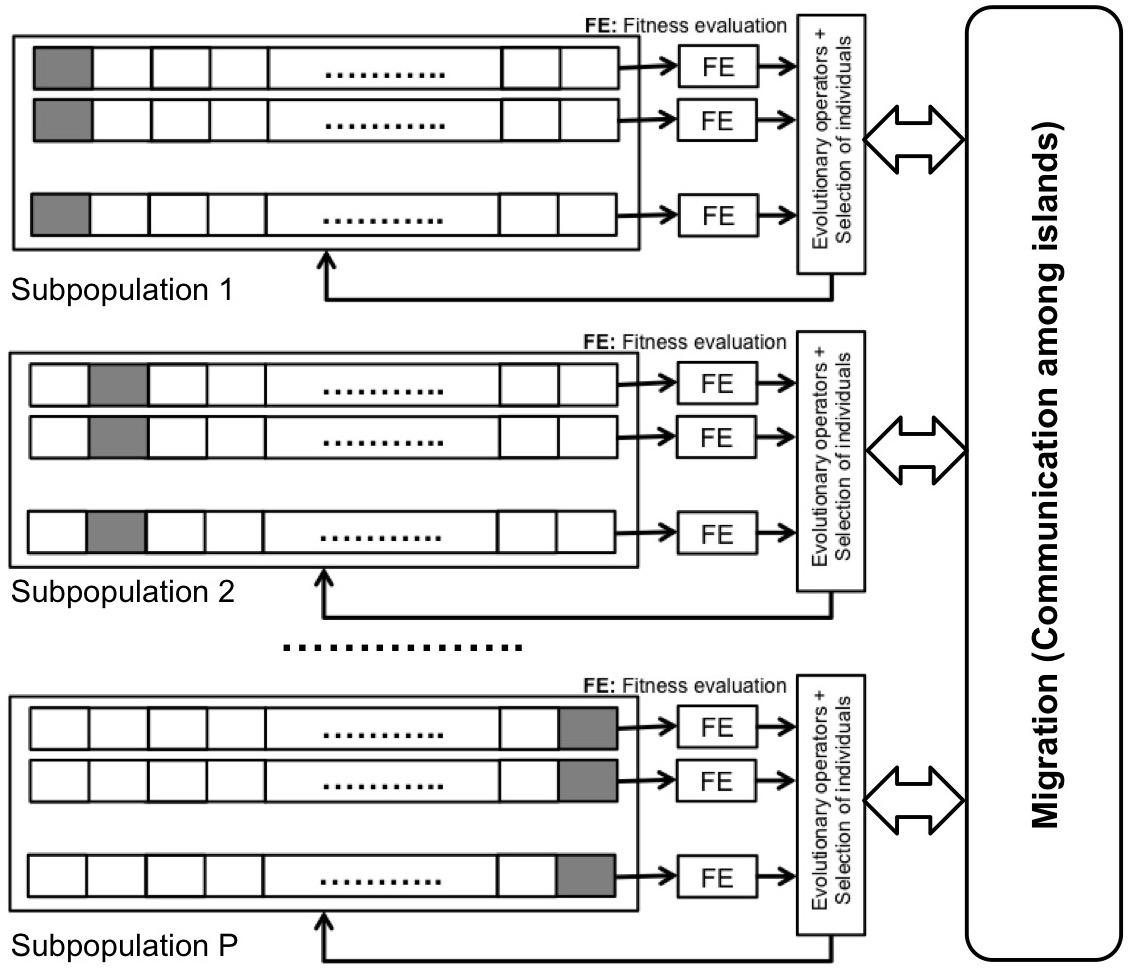
\includegraphics[width=12cm]{islandDisjoint.jpg}
%\caption{Disjoint algorithm: every island $p$ only modifies the $p_{th}$ components (in grey) of the individuals.}
%\label{fig:disjoint}
%\end{figure}
%
%\subsubsection{Coevolution with overlapping islands}
%This approach is similar to the previous one, but every island also
%uses the $p+1$ and $p-1$ (module size) chunks of the individual for
%crossover and migration. Therefore, some kind of overlapping of the
%crossed and mutated parts exists between islands. Figure
%\ref{fig:overlapping} shows the affected parts of the individuals in
%each island. 
%
% 
%\begin{figure}
%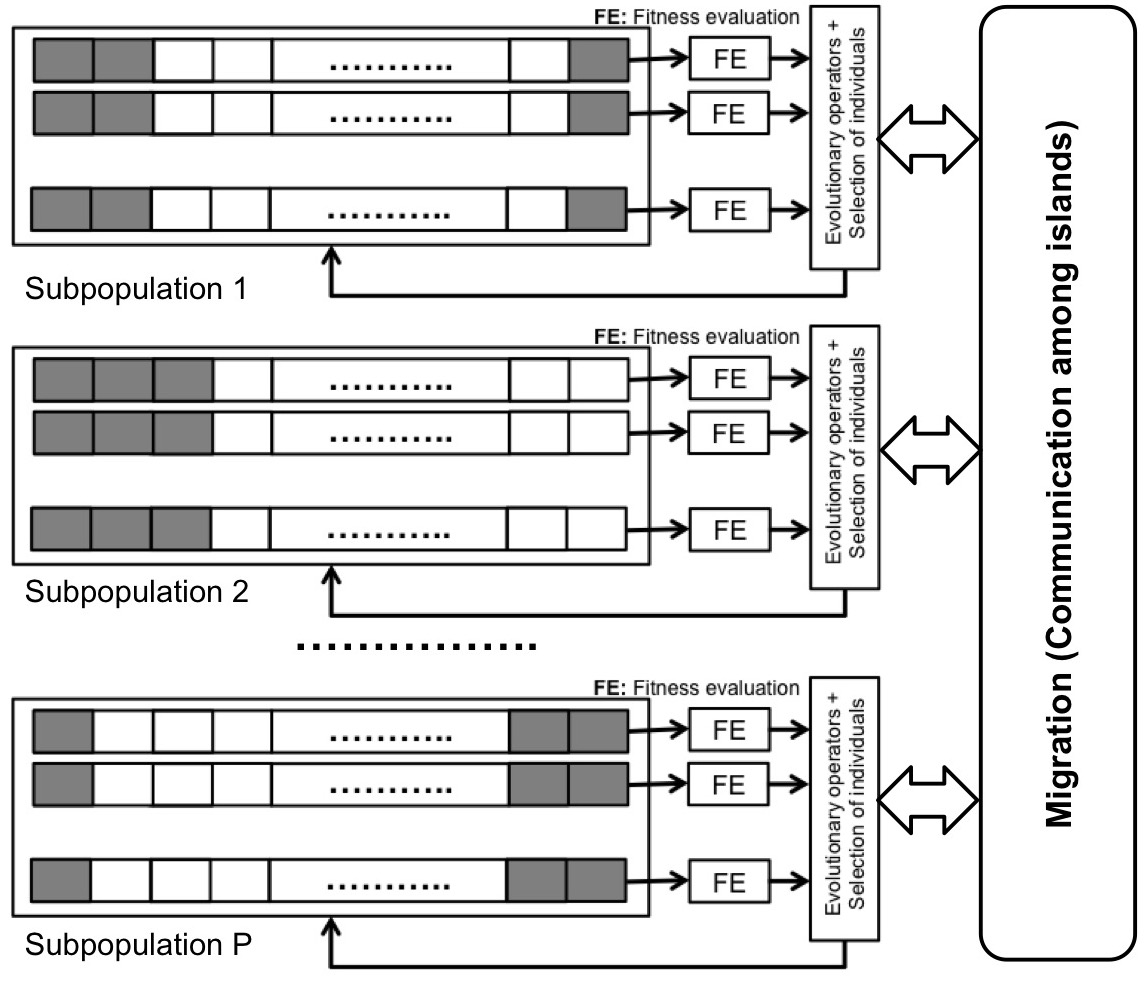
\includegraphics[width=12cm]{islandNoDisjoint.jpg}
%\caption{Overlapping algorithm: every island $p$ modifies the  $p+1$,
  %$p_{th}$ and $p-1$  components (in grey) of the individuals.}
%\label{fig:overlapping}
%\end{figure}

% --------------------------------------------------------------


%%%%%%%%%%%%%%%%%%%%%%%%%%  EXPERIMENTS AND RESULTS  %%%%%%%%%%%%%%%%%%%%%%%%%%
%
\section{Experiments and Results}
\label{sec:res}

%The three approaches have been run with two different 
%chromosome lengths ($L$): 512 and 2048. Different number of
%islands ($P$) have also been compared: 8, 32 and 128. This maximum number
%of islands have also been  used in previous work in the literature
%\cite{Martens13asynchronous}. The crossover and mutation chosen, SBX
%and polynomial, have been used previously by other authors in
%\cite{Durillo08masterslave}. 

%ZDT \cite{zdt2000a} has been chosen as a benchmark, since it is the most widely
%used in this area
%\cite{Deb03distributed,Martens13asynchronous,Wang09parallel,Durillo08masterslave}. The
%optimal PF distribution used for comparison has 1000
%solutions \footnote{Optimal PFs are available at:
%  \url{http://www.tik.ee.ethz.ch/sop/download/supplementary/testproblems/}.}. 





%The termination criterion used is the execution time: 25 seconds for dimension 512 and 100 (four times more) for 2048. We have used the time instead the number of evaluations firstly because our hypothesis argue that the time saved in crossover in mutation can be spent on improving the sub-populations and more operations and migrations can be achieved. Also, we are using different number of islands (with different sub-population sizes) that could lead to different execution times, so it would be difficult to compare different times and quality solutions at the same time.

\begin{table*}
\begin{center}
\begin{tabular}{|c|c|}
\hline
{\em Parameter Name} & {\em Value} \\ \hline
Number of islands ($P$) & 8, 32 and 128 \\ \hline
Chromosome size ($L$) & 512 and 2048 \\ \hline
Execution time (s) & 25 (for 512) and 100 (for 2048) \\ \hline \hline
Global population size ($N$) & 1024 \\ \hline
Selection type & Binary Tournament Selection \\ \hline
Replacement type & Generational \\ \hline 
Crossover type & SBX \\ \hline
Mutation  type & Polynomial\\ \hline
Mutation probability & 1/$L$ \\ \hline
Generations between migration & 5 \\ \hline
Individuals per migration & 1 \\ \hline
Selection for migration & Binary Tournament\\ \hline
Runs per configuration & 30 \\ \hline
\end{tabular}
\caption{Parameters and operators used in the experiments.}
\label{tab:parameters}
\end{center}
\end{table*}

The ECJ framework \cite{ECJ} has been used to run the
experiments. Specific operators have been developed as new modules for
ECJ, and they can be downloaded from our GitHub repository under a
LGPL V3 License
\footnote{\url{https://https://github.com/hpmoon/hpmoon-islands}}. The
island model has been executed synchronously, using the ECJ Internal
Island Model, in a CentOS 5.4 machine with Intel(R) Xeon(R) CPU E5520
@2.27GHz, 16 GB RAM, with Java Version 1.6.0\_16. As in this paper we
only focus on the behaviour of our model in a single machine scenario
(the islands share the same memory and processor), the migration time
will not be as important factor as in a real distributed system. This
task will be addressed in future works. %Pablo: no sé si decir esto
                                %aquí% 
%
%

%Different metrics, explained in the previous section, have been used to calculate the quality of the obtained PFs in each configuration. As some of the metrics require a reference point to be calculated (such as HV), the point (1,9) has been chosen as reference, as none of the generated PFs in all runs are dominated by it. Metrics are then normalized with respect to that point. A Kruskall-Wallis significance test has been performed to the metrics of all runs of the configurations, as the Kolmogorov-Smirnov test detected non-normal distributions. The average results for each configuration are shown in Table \ref{tab:results}.


\begin{table*}
\centering
\resizebox{12cm}{!}{
\begin{tabular}{|c||c|c|c|c||c|c|c|c||c|c|c|c||}
\hline
	&	\multicolumn{4}{|c|}{HV}													&	\multicolumn{4}{|c|}{Spread}														&	\multicolumn{4}{|c|}{IGD}														\\ \hline
%\multicolumn{13}{|c|}{2048 dimenOionO}																																													\\ \hline
\#Island	&	B		&	D		&	O			&	A			&	B		&	D			&	O			&	A			&	B		&	D		&	O		&	A					\\ \hline
\multicolumn{13}{|c|}{ZDT1}																																													\\ \hline
8	&	0.900		&	0.816		& \textbf{	0.926	}		&	Equiv. D			& \textbf{	0.729	}	&	1.041			&	0.898			&	Equiv. D			&	0.013		&	0.029		& \textbf{	0.007	}	&	Equiv. D					\\
16	& \textbf{	0.880	}	&	0.675		&	0.839			&	Equiv. O			& \textbf{	0.721	}	&	0.897			&	0.983		D	&	Equiv. O			& \textbf{	0.017	}	&	0.062		&	0.025		&	Equiv. O					\\
32	& \textbf{	0.829	}	&	0.618		&	0.698			&	0.790			& \textbf{	0.763	}	&	0.879			&	0.886		D	&	0.913	DO		& \textbf{	0.027	}	&	0.076		&	0.056		&	0.036					\\
64	& \textbf{	0.769	}	&	0.596		&	0.628			&	0.736			& \textbf{	0.820	}	&	0.897			&	0.872			&	0.890	DO		& \textbf{	0.040	}	&	0.080		&	0.071		&	0.047					\\
128	& \textbf{	0.707	}	&	0.585		&	0.598			&	0.668			& \textbf{	0.850	}	&	0.956			&	0.883			&	0.910	O		& \textbf{	0.053	}	&	0.083		&	0.079		&	0.062					\\ \hline
\multicolumn{13}{|c|}{ZDT2}																																													\\ \hline
8	&	0.830		&	0.786		& \textbf{	0.851	}		&	Equiv. D			& \textbf{	0.866	}	&	0.996			&	0.987		D	&	Equiv. D			&	0.023		&	0.037		& \textbf{	0.017	}	&	Equiv. D					\\
16	& \textbf{	0.810	}	&	0.601		&	0.776			&	Equiv. O			& \textbf{	0.916	}	&	0.990			&	1.005		D	&	Equiv. O			& \textbf{	0.029	}	&	0.091		&	0.040		&	Equiv. O					\\
32	& \textbf{	0.756	}	&	0.498		&	0.617			&	0.682			& \textbf{	0.976	}	& \textbf{	0.976	}	B	& \textbf{	0.978	}	BD	&	1.054			& \textbf{	0.045	}	&	0.119		&	0.086		&	0.068					\\
64	& \textbf{	0.668	}	&	0.451		&	0.504			&	0.601			&	1.002		& \textbf{	0.976	}		& \textbf{	0.974	}	D	&	1.025	B		& \textbf{	0.070	}	&	0.132		&	0.117		&	0.091					\\
128	& \textbf{	0.576	}	&	0.434		&	0.452			&	0.526			&	1.002		&	1.023			& \textbf{	0.978	}		&	1.015	BD		& \textbf{	0.096	}	&	0.137		&	0.132		&	0.110					\\ \hline
\multicolumn{13}{|c|}{ZDT3}																																													\\ \hline
8	&	0.928		&	0.838		& \textbf{	0.951	}		&	Equiv. D			& \textbf{	0.869	}	&	1.028			&	0.983		D	&	Equiv. D			& \textbf{	0.008	}	&	0.018		&	0.005		&	Equiv. D					\\
16	& \textbf{	0.903	}	&	0.715		&	0.870			&	Equiv. O			& \textbf{	0.846	}	&	0.899			&	0.960			&	Equiv. O			& \textbf{	0.011	}	&	0.032		&	0.014		&	Equiv. O					\\
32	& \textbf{	0.857	}	&	0.655		&	0.737			&	0.824			& \textbf{	0.845	}	&	0.879			&	0.873		D	&	0.881	DO		& \textbf{	0.016	}	&	0.039		&	0.030		&	0.019					\\
64	& \textbf{	0.796	}	&	0.632		&	0.662			&	0.761			& \textbf{	0.859	}	&	0.887			&	0.885		D	&	0.879	BDO		& \textbf{	0.023	}	&	0.042		&	0.038		&	0.027					\\
128	& \textbf{	0.738	}	&	0.620		&	0.633			&	0.705			& \textbf{	0.882	}	&	0.968			& \textbf{	0.888	}	B	&	0.911			& \textbf{	0.029	}	&	0.044		&	0.042		&	0.033					\\ \hline
\multicolumn{13}{|c|}{ZDT6}																																													\\ \hline
8	&	0.268		&	0.223		& \textbf{	0.298	}		&	Equiv. D			& \textbf{	0.988	}	& \textbf{	0.972	}	B	& \textbf{	0.996	}	B	&	Equiv. D			& \textbf{	0.173	}	&	0.191		&	0.160		&	Equiv. D					\\
16	& \textbf{	0.243	}	&	0.113		&	0.219			&	Equiv. O			& \textbf{	0.995	}	& \textbf{	0.987	}	B	& \textbf{	0.987	}	BD	&	Equiv. O			& \textbf{	0.184	}	&	0.240		&	0.193		&	Equiv. O					\\
32	& \textbf{	0.196	}	&	0.071		&	0.115			&	0.162			& \textbf{	0.998	}	& \textbf{	0.989	}	B	& \textbf{	0.988	}	BD	&	1.005	B		& \textbf{	0.204	}	&	0.257		&	0.238		&	0.220					\\
64	& \textbf{	0.145	}	&	0.056		&	0.075			&	0.120			&	0.996		&	0.986		B	& \textbf{	0.983	}	D	&	0.998	B		& \textbf{	0.226	}	&	0.264		&	0.255		&	0.235					\\
128	& \textbf{	0.104	}	&	0.049		&	0.055			&	0.084			&	0.993		&	1.007			& \textbf{	0.979	}		&	0.998	BD		& \textbf{	0.244	}	&	0.266		&	0.263		&	0.251					\\ \hline

\end{tabular}
}
\caption{Métricas de calidad obtenidas después de 30 ejecuciones por configuración, para los cuatro métodos comparados: baseline (B), disjunto (D), solapado (S) y solapado adaptativo (A). Los acrónimos junto a los valores indican que no hay diferencia significativa con respecto a ese método para ese valor. Los mejores valores están marcados en negrita.}
\label{tab:results512}
\end{table*}


\begin{table*}
\centering
\resizebox{12cm}{!}{
\begin{tabular}{|c||c|c|c|c||c|c|c|c||c|c|c|c||}
\hline
	&	\multicolumn{4}{|c|}{HV}													&	\multicolumn{4}{|c|}{Spread}														&	\multicolumn{4}{|c|}{IGD}														\\ \hline

\#Island	&	B		&	D		&	O			&	A			&	B		&	D			&	O			&	A			&	B		&	D		&	O		&	A					\\ \hline
\multicolumn{13}{|c|}{ZDT1}																																													\\ \hline
8	&	0.891		& \textbf{	0.953	}	&	0.937			&	Equiv. D			& \textbf{	0.681	}	& \textbf{	0.635	}	B	&	0.661		D	&	Equiv. D			&	0.015		& \textbf{	0.002	}	&	0.005		&	Equiv. D					\\
16	&	0.884		&	0.850		& \textbf{	0.942	}		&	Equiv. O			& \textbf{	0.705	}	&	0.908			& \textbf{	0.670	}	B	&	Equiv. O			&	0.016		&	0.022		& \textbf{	0.004	}	&	Equiv. O					\\
32	&	0.851		&	0.674		&	0.859		B	& \textbf{	0.900	}		& \textbf{	0.754	}	&	0.868			&	0.826		D	& \textbf{	0.763	}	B	&	0.023		&	0.062		&	0.020	B	& \textbf{	0.012	}				\\
64	& \textbf{	0.800	}	&	0.608		&	0.697			& \textbf{	0.824	}	B	& \textbf{	0.808	}	&	0.880			& \textbf{	0.861	}	B	& \textbf{	0.823	}	B	&	0.033		&	0.078		&	0.056		& \textbf{	0.027	}				\\
128	&	0.735		&	0.582		&	0.613			& \textbf{	0.745	}		& \textbf{	0.841	}	&	0.888			&	0.878		D	&	0.865		O	&	0.047		&	0.084		&	0.075		& \textbf{	0.043	}				\\ \hline
\multicolumn{13}{|c|}{ZDT2}																																													\\ \hline
8	&	0.832		& \textbf{	0.895	}	&	0.869			&	Equiv. D			& \textbf{	0.849	}	& \textbf{	0.886	}	B	&	0.853		D	&	Equiv. D			&	0.023		& \textbf{	0.006	}	&	0.013		&	Equiv. D					\\
16	&	0.831		&	0.833	B	& \textbf{	0.884	}		&	Equiv. O			& \textbf{	0.810	}	&	1.001			& \textbf{	0.802	}	B	&	Equiv. O			&	0.023		&	0.022	B	& \textbf{	0.009	}	&	Equiv. O					\\
32	&	0.800		&	0.628		&	0.800		B	& \textbf{	0.817	}		& \textbf{	0.848	}	&	0.974			&	0.983		D	&	0.908			&	0.031		&	0.082		&	0.032	B	& \textbf{	0.027	}				\\
64	& \textbf{	0.729	}	&	0.491		&	0.623			&	0.716			& \textbf{	0.909	}	&	0.967			&	0.979		D	& \textbf{	0.997	}	BD	& \textbf{	0.052	}	&	0.121		&	0.084		& \textbf{	0.055	}	B			\\
128	& \textbf{	0.630	}	&	0.441		&	0.500			& \textbf{	0.614	}	B	& \textbf{	0.957	}	&	0.989			&	0.978		D	& \textbf{	0.994	}	BO	& \textbf{	0.080	}	&	0.136		&	0.119		& \textbf{	0.085	}	B			\\ \hline
\multicolumn{13}{|c|}{ZDT3}																																													\\ \hline
8	&	0.917		& \textbf{	0.971	}	&	0.960			&	Equiv. D			& \textbf{	0.843	}	& \textbf{	0.854	}	B	&	0.868		D	&	Equiv. D			&	0.009		& \textbf{	0.001	}	&	0.004		&	Equiv. D					\\
16	&	0.911		&	0.876	B	& \textbf{	0.963	}		&	Equiv. O			& \textbf{	0.864	}	&	0.899		B	& \textbf{	0.837	}	B	&	Equiv. O			&	0.010		&	0.014		& \textbf{	0.003	}	&	Equiv. O					\\
32	&	0.884		&	0.710		&	0.883		B	& \textbf{	0.931	}		& \textbf{	0.856	}	& \textbf{	0.870	}	B	& \textbf{	0.842	}	B	& \textbf{	0.842	}	BDO	&	0.013		&	0.032		&	0.013	B	& \textbf{	0.008	}				\\
64	&	0.828		&	0.645		&	0.728			& \textbf{	0.854	}		& \textbf{	0.878	}	& \textbf{	0.896	}	B	& \textbf{	0.871	}	BD	& \textbf{	0.873	}	BDO	& \textbf{	0.019	}	&	0.040		&	0.030		& \textbf{	0.016	}	B			\\
128	& \textbf{	0.770	}	&	0.620		&	0.651			& \textbf{	0.773	}	B	& \textbf{	0.887	}	& \textbf{	0.901	}	B	& \textbf{	0.890	}	BD	& \textbf{	0.885	}	BDO	& \textbf{	0.026	}	&	0.043		&	0.039		& \textbf{	0.025	}	B			\\ \hline
\multicolumn{13}{|c|}{ZDT6}																																													\\ \hline
8	&	0.271		& \textbf{	0.398	}	&	0.323			&	Equiv. D			& \textbf{	0.982	}	& \textbf{	0.982	}	B	&	0.994			&	Equiv. D			&	0.171		& \textbf{	0.115	}	&	0.149		&	Equiv. D					\\
16	&	0.275		&	0.295	B	& \textbf{	0.354	}		&	Equiv. O			& \textbf{	0.981	}	& \textbf{	0.970	}	B	&	1.006			&	Equiv. O			&	0.170		&	0.161	B	& \textbf{	0.136	}	&	Equiv. O					\\
32	&	0.239		&	0.123		&	0.240			& \textbf{	0.254	}		& \textbf{	0.989	}	& \textbf{	0.991	}	B	& \textbf{	0.982	}	BD	& \textbf{	0.999	}	BD	&	0.186		&	0.235		&	0.185	B	& \textbf{	0.179	}				\\
64	& \textbf{	0.184	}	&	0.068		&	0.125			& \textbf{	0.178	}	B	& \textbf{	0.985	}	& \textbf{	0.982	}	B	& \textbf{	0.992	}	B	& \textbf{	0.995	}	BO	& \textbf{	0.209	}	&	0.259		&	0.235		&	0.212					\\
128	& \textbf{	0.128	}	&	0.051		&	0.071			& \textbf{	0.124	}	B	& \textbf{	0.991	}	& \textbf{	0.992	}	B	& \textbf{	0.988	}	BD	&	1.003			& \textbf{	0.233	}	&	0.266		&	0.257		& \textbf{	0.235	}	B			\\ \hline

\end{tabular}
}
\caption{Métricas de calidad obtenidas después de 30 ejecuciones por configuración, para los cuatro métodos comparados: baseline (B), disjunto (D), solapado (S) y solapado adaptativo (A). Los acrónimos junto a los valores indican que no hay diferencia significativa con respecto a ese método para ese valor. Los mejores valores están marcados en negrita.}
\label{tab:results512}
\end{table*}

%At a first glance results show that dividing the chromosome produces
%an improvement in all the quality indicators in all the
%configurations, with respect to the baseline. Also, results show that
%all the quality indicators lowers when the number of islands is
%increased, as the subpopulations are smaller. This is consistent with
%the claim by Durillo in \cite{Dorronsoro13superlinear}, who found that
%cooperative coevolutionary MOEAs work better on bigger populations
%(more than 100 individuals). Paying attention to the disjoint and
%overlapping methods, only when using 8 islands the disjoint method
%always attain better metrics, and even more times with the 2048 chromosome
%length. This can be explained because only 1/8 of the individual is
%changed in each island, while in the overlapping, 3/8 of the island
%may be more similar to the baseline configuration. Therefore, there exist some kind
%of limit point where one method will be preferable to another,
%depending the number of islands, population size and length. 
%
%This can be explained also comparing the number of generations and
%average solutions per island. Table \ref{tab:gens} shows these values
%obtained in each method. It is clear that in the same amount of time,
%the disjoint and overlapping method needs more generations than the
%baseline. This is even clearer with $L=$2048, where almost 10 times
%the number of generations is attained, and therefore, more migrations
%and crossovers/mutations can be achieved. Surprisingly, the average
%number of solutions of PFs per island in the baseline configuration is significantly
%higher in some configurations (mostly with 128 islands), but their
%combination in the final PF never attains higher values than Disjoint
%and Overlapping methods. 



\section{Conclusions}

%High-performance problems that require a large number of decision
%variables can leverage the division of the decision space that parallel
%and distributed algorithms imply. This can be done in dMOEAs by dividing the
%chromosome into different parts, each one modified by a different
%island. This paper compares a baseline distributed NSGA-II with two
%different strategies to separate the chromosome (disjoint or overlapping
%parts), using a high number of islands. Results show that these 
%methods can achieve better quality metrics
%than the baseline in the same amount of time. This can be explained 
%because of the time reduction in crossover and mutation in the chromosomes,
%producing a higher number of generations and more modifications of the 
%solutions of the PF in each sub-population, and therefore improving
%quality of the global PF.%

%Results also show that when increasing the number of islands, the overlapping 
%method significantly improves the results with respect to the disjoint method.
%Therefore, the relation between the number of islands used, the global population size,
%and the length of the chromosome may be a key factor to decide if using the 
%overlapping method or the disjoint one. Studying this factor with more types 
%of problems, and new configurations of population size and chromosome lengths will be addressed in the future.%
%

%Also, distributed implementations in several systems (such as a GRID or cluster) with more different
%quantities of islands/processors, will be used to perform a scalability study of the different
%methods, being the transmission time between islands a relevant issue to
%address. New benchmarks and real problems will also be  used to validate
%our approach. 



\begin{acks}
Acknowledgements
\end{acks}

\bibliographystyle{SageH}

\bibliography{hpmoon-hpca}
%\begin{thebibliography}{99}
%\bibitem[Kopka and Daly(2003)]{R1}
%Kopka~H and Daly~PW (2003) \textit{A Guide to \LaTeX}, 4th~edn.
%Addison-Wesley.%

%\bibitem[Lamport(1994)]{R2}
%Lamport~L (1994) \textit{\LaTeX: a Document Preparation System},
%2nd~edn. Addison-Wesley.%

%\bibitem[Mittelbach and Goossens(2004)]{R3}
%Mittelbach~F and Goossens~M (2004) \textit{The \LaTeX\ Companion},
%2nd~edn. Addison-Wesley.%

%\end{thebibliography}

\end{document}
